\chapter{Three Learning Principles}
\lecture{16}{28 Oct.}{}

\begin{prev}
    Validation (crossly) reserves validation data to simulate the testing
    procedure for model selection. Its guarantee rests on \(\Dval\) being
    drawn from the same distribution as the test data and never touched by
    the learning algorithm.
\end{prev}

Those two conditions are easy to state and easy to break. This chapter,
the last of the foundations, collects three principles that guard
them: prefer simple models (Occam's razor), make the data match the test
(sampling bias), and do not let the data shape the decisions they are meant
to judge (data snooping). It closes by looking back at the course in
threes.

\section{Occam's Razor}\label{sec:occam}

\source{slides p.2--6}

\subsection{Occam's Razor}

\begin{quote}
    \emph{An explanation of the data should be made as simple as possible,
    but no simpler.} --- Albert Einstein? (1879--1955)
\end{quote}

\begin{quote}
    \emph{entia non sunt multiplicanda praeter necessitatem} (entities must
    not be multiplied beyond necessity) --- William of Occam (1287--1347)
\end{quote}

\begin{center}
    
\includegraphics[width=3.2cm]{Figures/occam_razor.jpg}\\[2pt]
    {\scriptsize figure by Fred the Oyster (Own work) [CC-BY-SA-3.0], via
    Wikimedia Commons}
\end{center}

The question mark after Einstein is the deck's: the quote is commonly
attributed to him, but the attribution is doubtful. The second quote is the
original principle, and the razor in the picture is its metaphor.

\begin{moral}
    `Occam's razor' for trimming down unnecessary explanation.
\end{moral}

\subsection{Occam's Razor for Learning}

\begin{quote}
    \textbf{The simplest model that fits the data is also the most
    plausible.}
\end{quote}

\begin{center}
    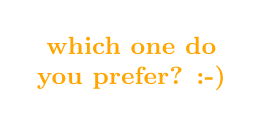
\begin{tikzpicture}[scale=1.1]
        \occamEllipse
        \node[font=\small\bfseries, text=Orange, align=center] at (3.5,0)
            {which one do\\you prefer? :-)};
        \begin{scope}[shift={(7,0)}]
            \occamBlobs
        \end{scope}
    \end{tikzpicture}
\end{center}

Both hypotheses separate the twenty examples of \autoref{sec:quad-hyp}
perfectly, so both have \(\Ein = 0\). The left one is a single ellipse,
\(x_1^2 + x_2^2 / 0.6 = 1\); the right one draws a small island around each
circle. Most people prefer the left one without hesitation. Two questions
make that preference precise:
\begin{enumerate}[(1)]
    \item What does it mean for a model to be simple?
    \item How do we know that simpler is better?
\end{enumerate}

\subsection{Simple Model}

\begin{center}
    \solidrules
    \begin{tabular}{p{0.4\textwidth}|p{0.4\textwidth}}
        \toprule
        \textbf{simple hypothesis} \(h\) & \textbf{simple model}
        \(\mathcal{H}\)\\
        \midrule
        \begin{itemize}[nosep, leftmargin=*, before=\vspace{-0.7\baselineskip}, after=\vspace{-\baselineskip}]
            \item small \(\Omega(h)\) \(=\) `looks' simple;
            \item specified by \textbf{few parameters}.
        \end{itemize}
        &
        \begin{itemize}[nosep, leftmargin=*, before=\vspace{-0.7\baselineskip}, after=\vspace{-\baselineskip}]
            \item small \(\Omega(\mathcal{H})\) \(=\) not many;
            \item contains a \textbf{small number of hypotheses}.
        \end{itemize}\\
        \bottomrule
    \end{tabular}
\end{center}

The two notions are the two complexities of \autoref{sec:reg-vc}:
\(\Omega(h)\) is the regularizer of a single hypothesis, \(\Omega(\mathcal{H})\)
the complexity of a whole set. They are connected:
\[
    h \text{ specified by } \ell \text{ bits} \Longleftarrow \abs{\mathcal{H}}
    \text{ of size } 2^\ell ,
    \qquad
    \text{small } \Omega(h) \Longleftarrow \text{small } \Omega(\mathcal{H}) .
\]
A set of \(2^\ell\) hypotheses can be indexed by \(\ell\) bits, so each of its
members is described by \(\ell\) bits only. A small set therefore contains
only hypotheses with short descriptions.

\begin{moral}
    Simple: \textbf{small hypothesis/model complexity}.
\end{moral}

\subsection{Simple is Better}

In addition to the math proof that you have seen (the VC bound), there is a
philosophical argument:
\[
    \begin{array}{rl}
        & \text{simple } \mathcal{H}\\
        \Longrightarrow & \text{smaller } m_{\mathcal{H}}(N)\\
        \Longrightarrow & \text{less `likely' to fit data perfectly:
        } \dfrac{m_{\mathcal{H}}(N)}{2^N}\\[8pt]
        \Longrightarrow & \text{more significant when fit happens.}
    \end{array}
\]
If the labels were random coin flips, each of the \(2^N\) labelings would be
equally likely, and only \(m_{\mathcal{H}}(N)\) of them can be fitted
perfectly by \(\mathcal{H}\). So \(\frac{m_{\mathcal{H}}(N)}{2^N}\) is the
probability that \(\mathcal{H}\) fits meaningless data perfectly. For a simple
\(\mathcal{H}\) this is tiny, so a perfect fit is strong evidence of a real
pattern; a complex \(\mathcal{H}\) fits almost anything, and its fit says
little.

\begin{center}
    \begin{tikzpicture}[scale=0.9]
        \occamEllipse
        \begin{scope}[shift={(3.4,0)}]
            \occamBlobs
        \end{scope}
    \end{tikzpicture}
\end{center}

\begin{moral}
    Direct action: \textbf{linear first}; always ask whether the \textbf{data
    are over-modeled}.
\end{moral}

\begin{exercise}[Fun Time]
    Consider the decision stumps in \(\mathbb{R}^1\) as the hypothesis set
    \(\mathcal{H}\). Recall that \(m_{\mathcal{H}}(N) = 2N\). Consider \(10\)
    different inputs \(x_1, x_2, \ldots, x_{10}\) coupled with labels \(y_n\)
    generated iid from a fair coin. What is the probability that the data
    \(\mathcal{D} = \{(x_n, y_n)\}_{n=1}^{10}\) is separable by
    \(\mathcal{H}\)?
    \begin{enumerate}[(1)]
        \item \(\frac{1}{1024}\);
        \item \(\frac{10}{1024}\);
        \item \(\frac{20}{1024}\);
        \item \(\frac{100}{1024}\).
    \end{enumerate}
\end{exercise}

\begin{proof}[Reference Answer]
    (3). Of all \(1024\) possible \(\mathcal{D}\), only \(2N = 20\) of them
    are separable by \(\mathcal{H}\). This is \(\frac{m_{\mathcal{H}}(N)}{2^N}\)
    of the previous subsection.
\end{proof}

\section{Sampling Bias}\label{sec:sampling-bias}

\source{slides p.7--12}

\subsection{Presidential Story}

\begin{itemize}
    \item In the 1948 US presidential election, Truman ran against Dewey.
    \item A newspaper ran a phone poll of how people voted, and set the
        headline `Dewey Defeats Truman' based on the polling.
\end{itemize}

\begin{center}
    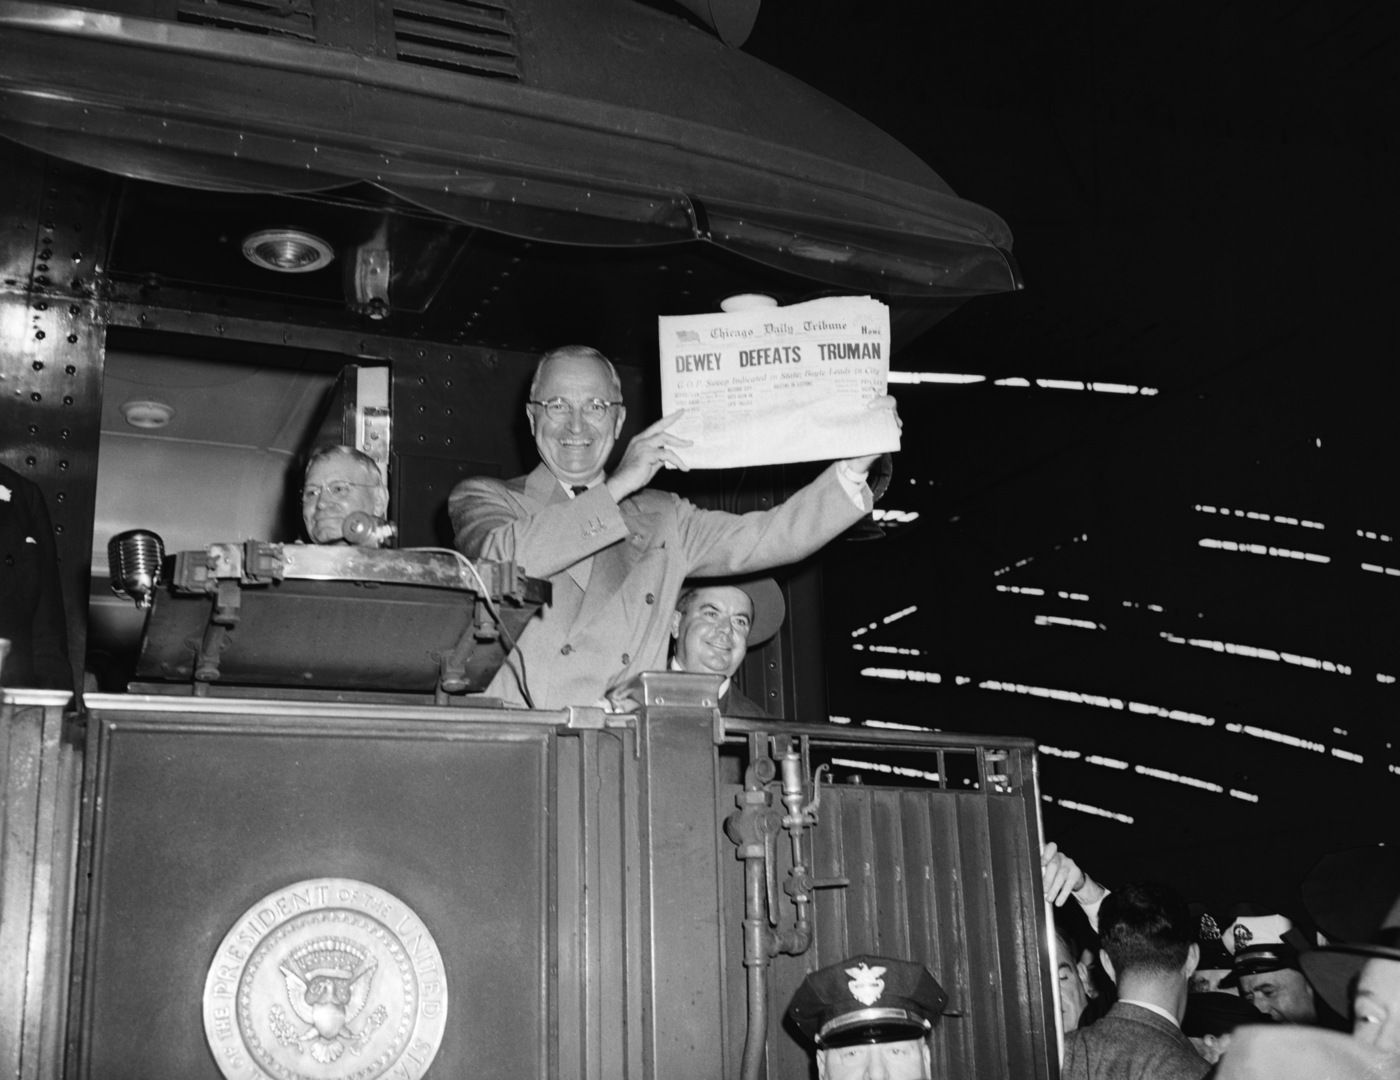
\includegraphics[width=6.4cm]{Figures/dewey_defeats_truman.jpg}
\end{center}

\begin{question}
    Who is this? :-)
\end{question}

\subsection{The Big Smile Came from \ldots}

The man holding up the newspaper is Truman, and yes, he won. So what went
wrong with the poll? Suspects of the mistake:
\begin{itemize}
    \item an editorial bug? No;
    \item bad luck of polling, the \(\delta\) of Hoeffding's inequality? No.
\end{itemize}

\begin{moral}
    Hint: phones were \textbf{expensive} :-)
\end{moral}

In 1948 mostly well-off households had a telephone, and they leaned towards
Dewey. The poll was a large and honest sample, but a sample of the wrong
population.

\subsection{Sampling Bias}

\begin{quote}
    \textbf{If the data is sampled in a biased way, learning will produce a
    similarly biased outcome.}
\end{quote}

\begin{itemize}
    \item Technical explanation: the data come from \(P_1(\bm{x}, y)\) but
        the test is under \(P_2 \neq P_1\), so the VC guarantee fails. The
        bound only relates \(\Ein\) to \(\Eout\) under the distribution that
        generated the data.
    \item Philosophical explanation: study Math hard but get tested on
        English, and there is no strong test guarantee.
\end{itemize}

\begin{moral}
    The `minor' VC assumption: data and testing are \textbf{both iid from
    \(P\)}.
\end{moral}

\subsection{Sampling Bias in Learning}

\paragraph{A true personal story.}
\begin{itemize}
    \item The Netflix competition for a movie recommender system offered
        \(1\) million US dollars for a \(10\%\) improvement.
    \item In the instructor's first shot, a \(\Dval\) was formed, and
        \(\Eval(g)\) showed a \(13\%\) improvement.
    \item Why am I still teaching here? :-)
\end{itemize}

\begin{center}
    \begin{adjustbox}{max width=0.75\textwidth}
        \recsysfactors
    \end{adjustbox}
\end{center}

The model was the factor-matching recommender of \autoref{sec:applications}.
The \(13\%\) did not survive the real test, because the validation set was
not built like the test set:

\begin{moral}
    Validation: \textbf{random examples} within \(\mathcal{D}\);\\
    test: \textbf{`last' user records} `after' \(\mathcal{D}\).
\end{moral}

Random validation examples are interleaved in time with the training ones,
so predicting them is easier than predicting a user's future ratings. The
validation set came from \(P_1\) and the test from \(P_2\).

\subsection{Dealing with Sampling Bias}

\begin{quote}
    \textbf{If the data is sampled in a biased way, learning will produce a
    similarly biased outcome.}
\end{quote}

\begin{itemize}
    \item Practical rule of thumb: \textbf{match the test scenario as much
        as possible}.
    \item For example, if the test uses the `last' user records `after'
        \(\mathcal{D}\):
        \begin{itemize}
            \item in training, \textbf{emphasize later examples}, as in
                KDDCup 2011;
            \item for validation, use the \textbf{`late' user records}.
        \end{itemize}
\end{itemize}

\begin{question}
    Last puzzle: what is the danger when learning `credit card approval' with
    \textbf{existing bank records}?
\end{question}

The bank only has repayment records for applicants it approved in the past.
The data are therefore sampled from approved customers, while the learned
\(g\) will be used on all applicants, including the kind the bank used to
reject.

\begin{exercise}[Fun Time]
    If the data \(\mathcal{D}\) is an unbiased sample from the underlying
    distribution \(P\) for binary classification, which of the following
    subset of \(\mathcal{D}\) is also an unbiased sample from \(P\)?
    \begin{enumerate}[(1)]
        \item all the positive (\(y_n > 0\)) examples;
        \item half of the examples that are randomly and uniformly picked from
            \(\mathcal{D}\) without replacement;
        \item half of the examples with the smallest \(\norm{\bm{x}_n}\)
            values;
        \item the largest subset that is linearly separable.
    \end{enumerate}
\end{exercise}

\begin{proof}[Reference Answer]
    (2). That's how we form the validation set, remember? :-) Each of the
    other three selects examples by their \(y_n\) or \(\bm{x}_n\), and so
    changes the distribution.
\end{proof}

\section{Data Snooping}\label{sec:data-snooping}

\source{slides p.13--17}

\subsection{Visual Data Snooping}

\begin{center}
    \begin{minipage}[c]{0.64\textwidth}
        Visualize \(\mathcal{X} = \mathbb{R}^2\):
        \begin{itemize}
            \item full \(\bm{\Phi}_2\): \(\bm{z} = (1, x_1, x_2, x_1^2, x_1
                x_2, x_2^2)\), \(\dvc = 6\);
            \item or \(\bm{z} = (1, x_1^2, x_2^2)\), \(\dvc = 3\),
                \textbf{after visualizing}?
            \item or better \(\bm{z} = (1, x_1^2 + x_2^2)\), \(\dvc = 2\)?
            \item or even better \(\bm{z} = \bigl( \sign(0.6 - x_1^2 - x_2^2)
                \bigr)\)?
        \end{itemize}
        --- careful about \textbf{your brain's `model complexity'}.
    \end{minipage}%
    \hfill
    \begin{minipage}[c]{0.32\textwidth}
        \centering
        \begin{tikzpicture}[scale=1.2]
            \fill[neghalf] (-1,-1) rectangle (1,1);
            \fill[poshalf] (0,0) circle ({sqrt(0.6)});
            \draw[sepline] (0,0) circle ({sqrt(0.6)});
            \circdataX
            \xplotframe
        \end{tikzpicture}
    \end{minipage}
\end{center}

This is the slide of \autoref{sec:visual-choices}, now with a name. Each
transform in the list was chosen after looking at the picture, and the small
\(\dvc\) it reports ignores the complexity of all the transforms the eye
tried and discarded.

\begin{moral}
    For VC-safety, \(\bm{\Phi}\) shall be decided \textbf{without `snooping'
    data}.
\end{moral}

\subsection{Data Snooping by Mere Shifting-Scaling}

\begin{quote}
    \textbf{If a data set has affected any step in the learning process, its
    ability to assess the outcome has been compromised.}
\end{quote}

Snooping does not need a picture. In the following experiment it hides in
the most innocent preprocessing step:
\begin{center}
    \begin{minipage}[c]{0.44\textwidth}
        \begin{itemize}
            \item There are \(8\) years of currency trading data.
            \item The first \(6\) years are for \textbf{training}, the last
                \(2\) years for \textbf{testing}.
            \item The input \(\bm{x}\) is the previous \(20\) days, the label
                \(y\) the \(21\)st day.
            \item Snooping versus no snooping: a superior profit is possible.
        \end{itemize}
    \end{minipage}%
    \hfill
    \begin{minipage}[c]{0.52\textwidth}
        \centering
        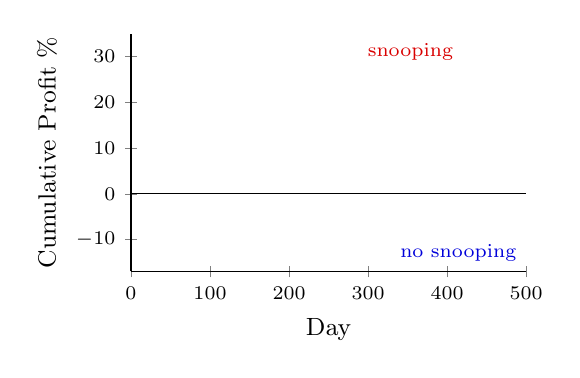
\begin{tikzpicture}
            \begin{axis}[width=6.6cm, height=4.6cm, xmin=0, xmax=500,
                ymin=-17, ymax=35, axis lines=left, axis line style={-},
                xtick={0,100,...,500}, ytick={-10,0,...,30},
                tick label style={font=\scriptsize},
                label style={font=\small}, xlabel={Day},
                ylabel={Cumulative Profit \%}, clip=false]
                \addplot[black, thin] coordinates {(0,0) (500,0)};
                \snoopProfitSnoop
                \snoopProfitClean
                \node[font=\scriptsize, text=red!85!black, anchor=east] at
                    (axis cs:420,31) {snooping};
                \node[font=\scriptsize, text=blue!85!black, anchor=south
                    east] at (axis cs:500,-16.8) {no snooping};
            \end{axis}
        \end{tikzpicture}
    \end{minipage}
\end{center}

\begin{itemize}
    \item Snooping: shift-scale all values by \textbf{training \(+\)
        testing}.
    \item No snooping: shift-scale all values by \textbf{training} only.
\end{itemize}

The only difference between the two runs is which days the mean and the
spread of the normalisation were computed from. With snooping, the
statistics of the test period leak into the training inputs, and the
`profit' over the \(500\) test days peaks near \(30\%\) and ends above
\(20\%\); done properly, the same model ends slightly below zero.

\subsection{Data Snooping by Data Reusing}

\paragraph{Research scenario.} On a benchmark data set \(\mathcal{D}\):
\begin{itemize}
    \item paper 1 proposes \(\mathcal{H}_1\) that works well on
        \(\mathcal{D}\);
    \item paper 2 finds room for improvement and proposes \(\mathcal{H}_2\),
        and is published only if \(\mathcal{H}_2\) is better than
        \(\mathcal{H}_1\) on \(\mathcal{D}\);
    \item paper 3 finds room for improvement and proposes \(\mathcal{H}_3\),
        and is published only if \(\mathcal{H}_3\) is better than
        \(\mathcal{H}_2\) on \(\mathcal{D}\);
    \item \ldots
\end{itemize}

What is wrong:
\begin{itemize}
    \item If all papers came from the same author as one big paper, it would
        be one learning algorithm on \(\bigcup_m \mathcal{H}_m\), with bad
        generalization due to \(\dvc(\cup_m \mathcal{H}_m)\).
    \item Step-wise, the later authors \textbf{snooped} the data by reading
        the earlier papers, and the bad generalization is worsened by
        \textbf{publish only if better}, which is a selection on
        \(\mathcal{D}\) itself.
\end{itemize}

\begin{moral}
    If you torture the data long enough, it will confess :-)
\end{moral}

\subsection{Dealing with Data Snooping}

\begin{itemize}
    \item Truth: it is very hard to avoid, unless one is extremely honest.
    \item Extremely honest: lock your test data in a safe.
    \item Less honest: reserve validation data and use them cautiously.
\end{itemize}
Beyond these:
\begin{itemize}
    \item Be blind: avoid making modeling decisions by looking at the data.
    \item Be suspicious: interpret research results, including your own, with
        a proper feeling of contamination.
\end{itemize}

\begin{moral}
    One secret to winning KDDCups: a careful balance between data-driven
    modeling (snooping) and validation (no-snooping).
\end{moral}

Some snooping is unavoidable in practice, since looking at the data is how
good features are found. The point is to pay for it with an honest
validation step that the snooping never touched.

\begin{exercise}[Fun Time]
    Which of the following can result in unsatisfactory test performance in
    machine learning?
    \begin{enumerate}[(1)]
        \item data snooping;
        \item overfitting;
        \item sampling bias;
        \item all of the above.
    \end{enumerate}
\end{exercise}

\begin{proof}[Reference Answer]
    (4). A professional like you should be aware of those! :-)
\end{proof}

\section{Power of Three}\label{sec:power-of-three}

\source{slides p.18--24}

The course so far, reviewed in groups of three.

\subsection{Three Related Fields}

\begin{center}
    \solidrules
    \begin{tabular}{*{2}{>{\raggedright\arraybackslash}p{0.28\textwidth}|}>{\raggedright\arraybackslash}p{0.28\textwidth}}
        \toprule
        \textbf{Data Mining} & \textbf{Artificial Intelligence} &
        \textbf{Statistics}\\
        \midrule
        \begin{itemize}[nosep, leftmargin=*, before=\vspace{-0.7\baselineskip}, after=\vspace{-\baselineskip}]
            \item use (huge) data to \textbf{find property} that is
                interesting;
            \item difficult to distinguish ML and DM in reality.
        \end{itemize}
        &
        \begin{itemize}[nosep, leftmargin=*, before=\vspace{-0.7\baselineskip}, after=\vspace{-\baselineskip}]
            \item compute something that shows \textbf{intelligent
                behavior};
            \item ML is one possible route to realize AI.
        \end{itemize}
        &
        \begin{itemize}[nosep, leftmargin=*, before=\vspace{-0.7\baselineskip}, after=\vspace{-\baselineskip}]
            \item use data to \textbf{make inference} about an unknown
                process;
            \item statistics contains many useful tools for ML.
        \end{itemize}\\
        \bottomrule
    \end{tabular}
\end{center}

These are the neighbours of \autoref{sec:other-fields}.

\subsection{Three Theoretical Bounds}

\begin{center}
    \solidrules
    \begin{tabular}{*{2}{>{\raggedright\arraybackslash}p{0.28\textwidth}|}>{\raggedright\arraybackslash}p{0.28\textwidth}}
        \toprule
        \textbf{Hoeffding} & \textbf{Multi-Bin Hoeffding} & \textbf{VC}\\
        \midrule
        \(\begin{aligned} & \mathbb{P}[\text{BAD}]\\ \le {} & 2
        \exp(-2\epsilon^2 N) \end{aligned}\)
        &
        \(\begin{aligned} & \mathbb{P}[\text{BAD}]\\ \le {} & 2M
        \exp(-2\epsilon^2 N) \end{aligned}\)
        &
        \(\begin{aligned} & \mathbb{P}[\text{BAD}]\\ \le {} & 4
        m_{\mathcal{H}}(2N) \exp(\ldots) \end{aligned}\)\\[14pt]
        \begin{itemize}[nosep, leftmargin=*, before=\vspace{-0.7\baselineskip}, after=\vspace{-\baselineskip}]
            \item \textbf{one} hypothesis;
            \item useful for \textbf{verifying/testing}.
        \end{itemize}
        &
        \begin{itemize}[nosep, leftmargin=*, before=\vspace{-0.7\baselineskip}, after=\vspace{-\baselineskip}]
            \item \(M\) hypotheses;
            \item useful for \textbf{validation}.
        \end{itemize}
        &
        \begin{itemize}[nosep, leftmargin=*, before=\vspace{-0.7\baselineskip}, after=\vspace{-\baselineskip}]
            \item all \(\mathcal{H}\);
            \item useful for \textbf{training}.
        \end{itemize}\\
        \bottomrule
    \end{tabular}
\end{center}

They are \autoref{thm:hoeffding-h}, \autoref{thm:finite-hoeffding} and
\autoref{thm:vc}. Each bound pays for exactly the amount of choice that was
made: none when a fixed \(g\) is tested, \(M\) when one of \(M\) finalists is
validated, and the growth function when \(g\) is trained from all of
\(\mathcal{H}\).

\subsection{Three Linear Models}

\begin{center}
    \begin{adjustbox}{max width=\textwidth}
        \solidrules
        \begin{tabular}{@{}c|c|c@{}}
            \toprule
            \textbf{PLA/pocket} & \textbf{linear regression}
            & \textbf{logistic regression}\\
            \(h(\bm{x}) = \sign(s)\) & \(h(\bm{x}) = s\)
            & \(h(\bm{x}) = \theta(s)\)\\
            \midrule
            \scoreunit{sign} & \scoreunit{id} & \scoreunit{theta}\\[4pt]
            plausible \(\err\) \(=\) 0/1 & friendly \(\err\) \(=\) squared
            & plausible \(\err\) \(=\) CE\\
            \textcolor{blue!80!black}{(small flipping noise)}
            & \textcolor{blue!80!black}{(easy to minimize)}
            & \textcolor{blue!80!black}{(maximum likelihood)}\\
            minimize \textbf{specially} & minimize \textbf{analytically}
            & minimize \textbf{iteratively}\\
            \bottomrule
        \end{tabular}
    \end{adjustbox}
\end{center}

This completes the table of \autoref{sec:logreg-problem}, whose third error
measure was still a question mark there. The last row is how each one is
optimized: PLA and pocket by their special update rules, linear regression by
the pseudo-inverse, logistic regression by gradient descent.

\subsection{Three Key Tools}

\begin{center}
    \solidrules
    \begin{tabular}{*{2}{>{\raggedright\arraybackslash}p{0.28\textwidth}|}>{\raggedright\arraybackslash}p{0.28\textwidth}}
        \toprule
        \textbf{Feature Transform} & \textbf{Regularization} &
        \textbf{Validation}\\
        \midrule
        \(\begin{aligned} \Ein(\bm{w}) &\to \Ein(\tilde{\bm{w}})\\
        \dvc(\mathcal{H}) &\to \dvc(\mathcal{H}_{\bm{\Phi}}) \end{aligned}\)
        &
        \(\begin{aligned} \Ein(\bm{w}) &\to \Ein(\wreg)\\
        \dvc(\mathcal{H}) &\to \deff(\mathcal{H}, \mathcal{A}) \end{aligned}\)
        &
        \(\begin{aligned} \Ein(h) &\to \Eval(h)\\
        \mathcal{H} &\to \{g_1^-, \ldots, g_M^-\} \end{aligned}\)\\[14pt]
        \begin{itemize}[nosep, leftmargin=*, before=\vspace{-0.7\baselineskip}, after=\vspace{-\baselineskip}]
            \item by using a \textbf{more complicated} \(\bm{\Phi}\);
            \item \textbf{lower} \(\Ein\);
            \item higher \(\dvc\).
        \end{itemize}
        &
        \begin{itemize}[nosep, leftmargin=*, before=\vspace{-0.7\baselineskip}, after=\vspace{-\baselineskip}]
            \item by \textbf{augmenting regularizer} \(\Omega\);
            \item \textbf{lower} \(\deff\);
            \item higher \(\Ein\).
        \end{itemize}
        &
        \begin{itemize}[nosep, leftmargin=*, before=\vspace{-0.7\baselineskip}, after=\vspace{-\baselineskip}]
            \item by reserving \(K\) examples as \(\Dval\);
            \item \textbf{fewer choices};
            \item fewer examples.
        \end{itemize}\\
        \bottomrule
    \end{tabular}
\end{center}

Each tool moves one of the two terms of the VC bound \(\Eout \le \Ein +
\Omega\) at the expense of the other, which is why each column lists one
gain (in bold) and one price.

\subsection{Three Learning Principles}

\begin{center}
    \solidrules
    \begin{tabular}{*{2}{>{\raggedright\arraybackslash}p{0.28\textwidth}|}>{\raggedright\arraybackslash}p{0.28\textwidth}}
        \toprule
        \textbf{Occam's Razor} & \textbf{Sampling Bias} & \textbf{Data
        Snooping}\\
        \midrule
        simple is good & class matches exam & honesty is best policy\\
        \bottomrule
    \end{tabular}
\end{center}

\subsection{Three Future Directions}

\begin{center}
    \solidrules
    \begin{tabular}{*{2}{>{\raggedright\arraybackslash}p{0.28\textwidth}|}>{\raggedright\arraybackslash}p{0.28\textwidth}}
        \toprule
        \textbf{More Transform} & \textbf{More Regularization} & \textbf{Less
        Label}\\
        \bottomrule
    \end{tabular}
\end{center}

\begin{center}
    \begin{adjustbox}{max width=\textwidth}
        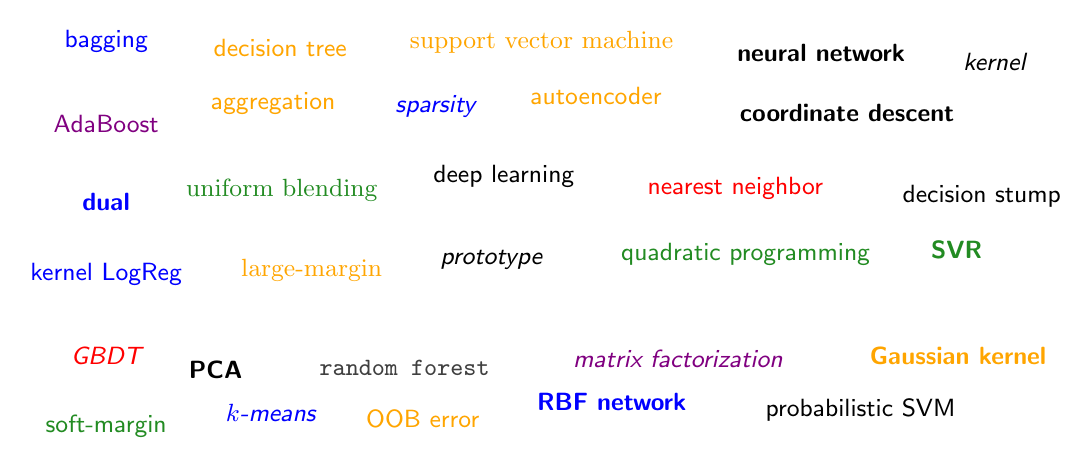
\begin{tikzpicture}[font=\small\sffamily,
            w/.style={inner sep=1pt}]
            \node[w, text=blue] at (1.50,-0.29) {bagging};
            \node[w, text=Orange] at (3.71,-0.37) {decision tree};
            \node[w, text=Orange, font=\small\rmfamily] at (7.03,-0.30)
                {support vector machine};
            \node[w, font=\small\sffamily\bfseries] at (10.58,-0.44)
                {neural network};
            \node[w, font=\small\sffamily\itshape] at (12.78,-0.55) {kernel};
            \node[w, text=Purple] at (1.50,-1.33) {AdaBoost};
            \node[w, text=Orange] at (3.62,-1.08) {aggregation};
            \node[w, text=blue, font=\small\sffamily\itshape] at (5.68,-1.11)
                {sparsity};
            \node[w, text=Orange] at (7.72,-0.98) {autoencoder};
            \node[w, font=\small\sffamily\bfseries] at (10.91,-1.20)
                {coordinate descent};
            \node[w, text=blue, font=\small\sffamily\bfseries] at
                (1.50,-2.33) {dual};
            \node[w, text=ForestGreen, font=\small\rmfamily] at (3.73,-2.18)
                {uniform blending};
            \node[w] at (6.55,-2.00) {deep learning};
            \node[w, text=red] at (9.49,-2.15) {nearest neighbor};
            \node[w] at (12.62,-2.26) {decision stump};
            \node[w, text=blue] at (1.50,-3.24) {kernel LogReg};
            \node[w, text=Orange, font=\small\rmfamily] at (4.11,-3.20)
                {large-margin};
            \node[w, font=\small\sffamily\itshape] at (6.39,-3.06)
                {prototype};
            \node[w, text=ForestGreen] at (9.62,-2.99) {quadratic
                programming};
            \node[w, text=ForestGreen, font=\small\sffamily\bfseries] at
                (12.30,-2.93) {SVR};
            \node[w, text=red, font=\small\sffamily\itshape] at (1.50,-4.28)
                {GBDT};
            \node[w, font=\small\sffamily\bfseries] at (2.89,-4.46) {PCA};
            \node[w, text=black!75, font=\small\ttfamily] at (5.29,-4.44)
                {random forest};
            \node[w, text=Purple, font=\small\sffamily\itshape] at
                (8.76,-4.32) {matrix factorization};
            \node[w, text=Orange, font=\small\sffamily\bfseries] at
                (12.32,-4.28) {Gaussian kernel};
            \node[w, text=ForestGreen] at (1.50,-5.18) {soft-margin};
            \node[w, text=blue, font=\small\sffamily\itshape] at (3.59,-5.01)
                {\(k\)-means};
            \node[w, text=Orange] at (5.52,-5.08) {OOB error};
            \node[w, text=blue, font=\small\sffamily\bfseries] at
                (7.92,-4.86) {RBF network};
            \node[w] at (11.08,-4.97) {probabilistic SVM};
        \end{tikzpicture}
    \end{adjustbox}
\end{center}

The three headings name the directions the course continues in: richer
transforms, stronger or smarter regularization, and learning with fewer
labels. The cloud below them is the vocabulary of the techniques to come,
from support vector machines and kernels to aggregation, decision trees and
deep learning.

\begin{moral}
    Ready for the \textbf{jungle}!
\end{moral}

\begin{exercise}[Fun Time]
    What are the magic numbers that repeatedly appear in this class?
    \begin{enumerate}[(1)]
        \item \(3\);
        \item \(1126\);
        \item both \(3\) and \(1126\);
        \item neither \(3\) nor \(1126\).
    \end{enumerate}
\end{exercise}

\begin{proof}[Reference Answer]
    (3). \(3\) as illustrated, and you may recall \(1126\) somewhere :-)
\end{proof}

\hrulebar

\subsection*{Summary}

\begin{description}
    \item[Occam's Razor] simple, simple, simple!
    \item[Sampling Bias] match test scenario as much as possible.
    \item[Data Snooping] any use of data is `contamination'.
    \item[Power of Three] relatives, bounds, models, tools, principles.
\end{description}

These principles close the four parts of the foundations: when machines can
learn, why, how, and how to learn better. Next: ready for the jungle!
